\documentclass[11pt]{article}
\usepackage{../cs70,latexsym,epsf}
\lecture{18}
\def\title{Note \the\lecturenumber}

\newcommand{\pop}{\text{pop}}
\newcommand{\freq}{\text{freq}}
\newcommand{\inc}{\text{inc}}

\begin{document}
\maketitle

\section*{Zipf's Law and Power Law Distributions}


A random graph with $n$ nodes is created by the following process: For each pair of nodes $i$ and $j$, the edge $\{i,j\}$ is present with probability $p = \frac{d}{n}$, independently of the other edges. So each edge can be modeled as a biased coin flip. From the point of view of a node, the edges adjacent to this node are distributed according to a binomial distribution with mean $(n-1) \cdot \frac{d}{n} \approx d$ and variance $(n-1) \cdot \frac{d}{n} \cdot (1-\frac{d}{n}) \approx d$ (assuming $n \gg d$).

We know that the binomial distribution (like all distributions we have seen so far) is very concentrated about the mean. For example, if a graph with $n = $ 20,000 nodes has average degree $d = 4$, then we do not expect any node to have degree 20 or more, since that probability is exponentially small. But in the Internet, the graph of the 20,000 or so autonomous systems which indeed has average degree near 4, it turns out there are about 40 nodes that have degree greater than 20. And in the www (the graph of hyperlinks between $n = $ 10,000,000 documents, if we ignore directions), which is a graph with average degree about 12, more than 100,000 have degree at least 100.

We must conclude that there is some kind of dependence between the edges of these graphs, that they came about by a process that is very different from independent coin tosses we considered above. The degrees of these graphs seem to have a density function that does not decrease exponentially with the difference from the mean.

\subsection*{Zipf's Law}

George Kingsley Zipf was a linguist who studied the statistical properties of languages. He noticed that the occurrences of the most frequent words in English (and in other languages) follow a particular pattern. If the most frequent word appears $N$ times in a corpus (say, Shakespeare's plays), then the second most frequent word appears approximately $\frac{N}{2}$ times, and the third most frequent word appears approximately $\frac{N}{3}$ times, and so on. In general, if $\freq_i$ denotes the frequency of the $i$-th most frequent word, then we find that
$$\freq_i \approx \frac{\freq_1}{i}.$$
This phenomenon is quite pervasive, and it is called {\em Zipf's Law}. 

Another place where this law appears is in the population of cities. The largest city of the USA is New York, which has population $\pop_1 \approx $ 8,000,000. The second largest city, Los Angeles, has population $\pop_2 \approx$ 3,800,000, while the third largest city, Chicago, has population $\pop_3 \approx$ 2,700,000, and so on. In general, if $\pop_i$ denotes the population of the $i$-th largest city, then we also find the same relationship:
$$\pop_i \approx \frac{\pop_1}{i}.$$
This means if we plot $\log(\pop_i)$ as a function of $\log(i)$, then we notice that it is almost a straight line with angle 45\%; see Figure~\ref{fig:cities} for an illustration.\footnote{Figure is taken from: Xavier Garbaix, {\em ``Zipf's Law for Cities: An Explanation''}, The Quarterly Journal of Economics, 1999.}

\begin{figure}[h!]
\centering
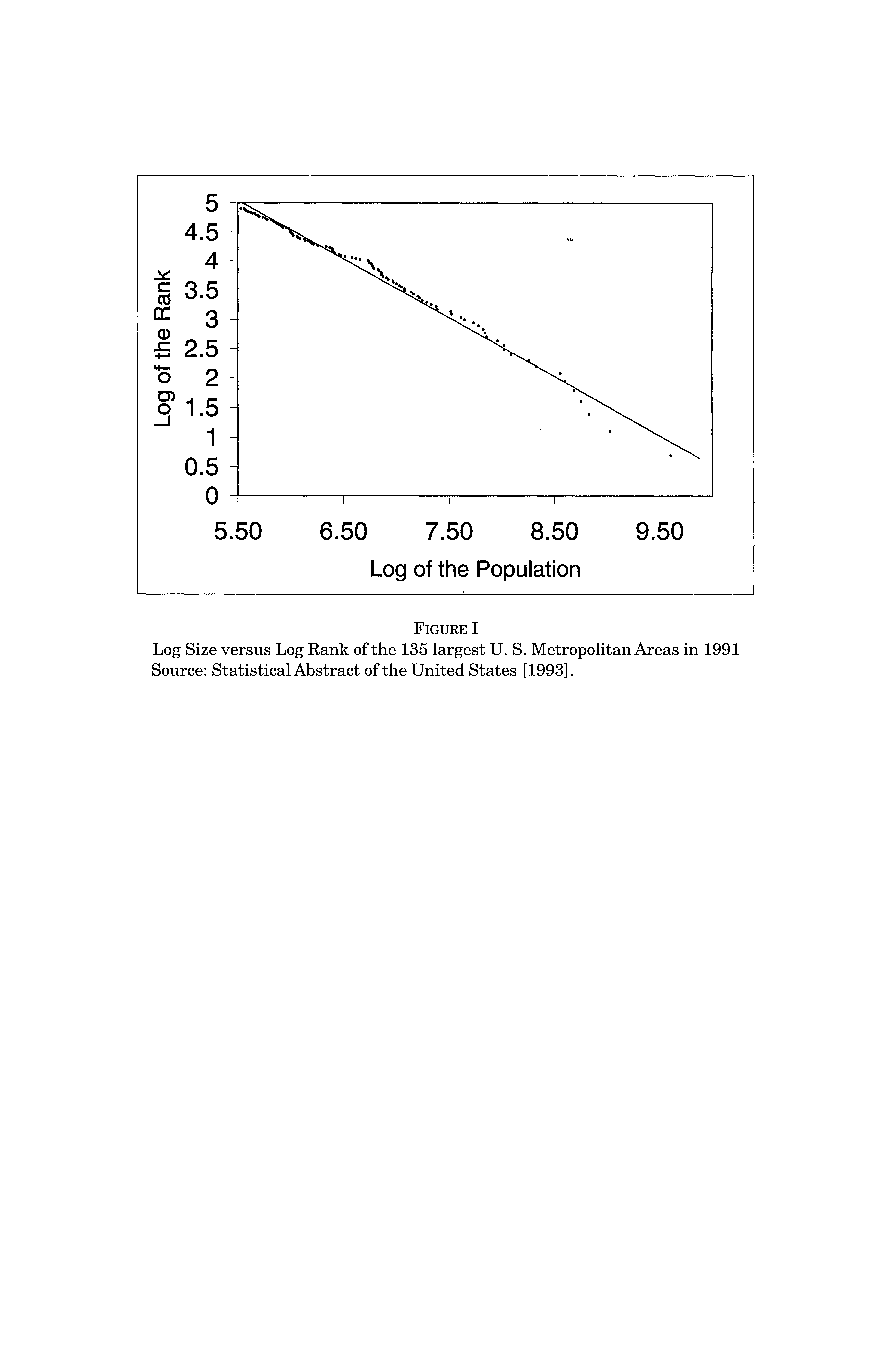
\includegraphics[scale=0.8]{cities}
\caption{Log-log plot of the population of the largest cities. Straight line indicates power law distribution.}
\label{fig:cities}
\end{figure}


\subsection*{Power Laws}

There is a similar phenomenon in the distribution of incomes, first observed by the economist Pareto. He noticed that
\begin{equation}\label{Eq:PowerLaw}
\Pr(\text{income} \ge x) = \frac{D}{x^{\alpha-1}}
\end{equation}
for some constant $D$ and power $\alpha$. This means among a population of $N$ individuals,
$$\frac{\#\text{ of people with income } \ge x}{N} ~=~ \frac{D}{x^{\alpha-1}}.$$
In particular, the highest income $\inc_1$ is the value of $x$ such that there is only $1$ person with that income:
$$\frac{1}{N} ~=~ \frac{D}{\inc_1^{\alpha-1}} ~~~\Leftrightarrow~~~ \inc_1 = (ND)^{1/(\alpha-1)}.$$
And in general, the $i$-th highest income $\inc_i$ is the value of $x$ such that there are $i$ people with income $\ge x$:
$$\frac{i}{N} ~=~ \frac{D}{\inc_1^{\alpha-1}} ~~~\Leftrightarrow~~~ \inc_i = \left(\frac{ND}{i}\right)^{1/(\alpha-1)}.$$
Substituting the value $\inc_i = (ND)^{1/(\alpha-1)}$ and letting $\beta = \frac{1}{\alpha-1}$ for simplicity, we get the relationship:
$$\inc_i ~=~ \frac{\inc_1}{i^\beta}.$$
This kind of distribution is called a {\em power law}. We see that Zipf's Law is the special case $\beta = 1$ (or $\alpha = 2$), but in general the power $\beta$ can be arbitrary. In practice, we try to find the best value of $\beta$ that fits our data.


\medskip
{\bf Heavy tail.}~The density function of the power law distribution, which is obtained by differentiating~\eqref{Eq:PowerLaw}, is
$$f(x) = \frac{D(\alpha-1)}{x^\alpha}.$$
Notice that it decreases {\em polynomially}, not exponentially, with $x$. Contrast this with the other distributions that we have seen previously. For example, the exponential distribution has density
$$f_{\text{Exp}}(x) = \lambda e^{-\lambda x},$$
which decreases exponentially with $x$, while the normal distribution has density
$$f_{\text{Normal}}(x) = \frac{1}{\sqrt{2\pi\sigma^2}} \exp\left(-\frac{(x-\mu)^2}{2\sigma^2}\right),$$
which decreases exponentially with $x^2$ as we move away from the mean $\mu$. On the other hand, the power law density only decreases polynomially, which is much slower. Figure~\ref{fig:tails} shows a comparison of the polynomial and exponential decreases (we shift the exponential functions so they all start at the same point).

\begin{figure}[h!]
\centering
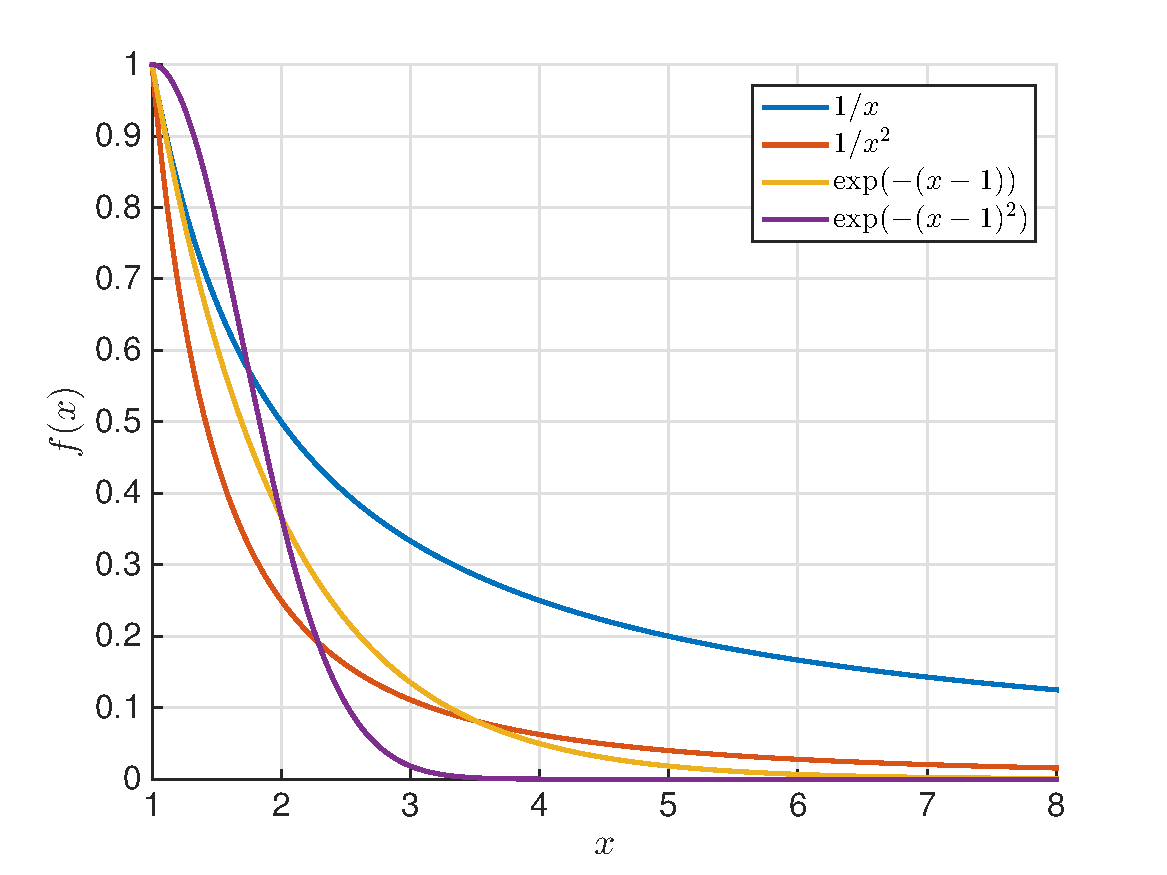
\includegraphics[scale=0.4]{tails}
\caption{Comparison of the polynomial vs.\ exponential decrease.}
\label{fig:tails}
\end{figure}

Similarly, the tail probability~\eqref{Eq:PowerLaw} itself is also decreasing polynomially with $x$. On the other hand, the other distributions that we have seen so far (binomial, normal, Poisson, geometric, and exponential) all have tail probabilities that are decreasing exponentially with $x$. For this reason, power law distributions are often called {\em ``heavy tailed''} distributions (the tail probability is larger than normal or other distributions).


\medskip
{\bf Where do power laws come from?}~
We know that the exponentially concentrated distributions are produced by many independent contributions (as in the binomial distribution, or the normal distribution, viz.~the law of large numbers). What kind of processes produce power law distributions? In general, power law distributions typically appear in phenomena related to human activities. There are several processes that are known to produce such distributions:
\begin{itemize}
  \item {\bf Size-independent growth:} If the ratio of a person's income next year to this year's income is a random variable that does not depend on the income, then it can be shown that, after a while, a population whose incomes evolve this way will obey a power law. This is how a network evolves: high-degree nodes are ``important,'' and attract more edges.
  
  \item {\bf Trade-offs:} If people try to optimize a single objective, then concentrated distributions often result. But if they must optimize --- trade one against the other --- two or more objectives simultaneously, then the optimum usually has power law-distributed features. Entities interacting in a complicated environment like the Internet and the www are likely to behave this way.
  
  \item {\bf Imitation or copying:} Consider the number of citations that a paper receives. When people write research papers and they need to find a citation for some topic, they typically look at the literature and see what paper is usually cited for that topic, which results in that paper getting more citations. This imitation or copying process results in a power law distribution.
  
  \item {\bf Preferential attachment:} The web is arguably constructed by new documents creating hyperlinks to documents discovered by following other hyperlinks. If a document has many links attached to it, then it is more likely to be discovered, and in turn it is more likely to receive more links. Thus, popular documents are likely to become more popular, a phenomenon informally called {\em ``the rich gets richer.''} This results in a power law distribution.
\end{itemize}


\subsection*{Polya Urn}

There is a simple model that captures the essence of preferential attachment. Suppose that you have two bins, the white and the black bin, with $w$ and $b$ balls inside, respectively, and you throw a new ball. The balls are magnetic, and they attract the new ball with force proportional to their number; so the new ball will go to the white bin with probability $\frac{w}{w+b}$.

Suppose we start with $w = b = 1$, and throw in $n$ new balls one at a time. How is the resulting distribution going to look like? This process is called a {\em Polya urn}. Intuitively, the ``attraction'' rule is going to enhance inequalities, so the bins are not going to be very load-balanced. But how exactly?

For example, what is the probability that, if we throw in 1,000 balls, there will be 900 or more balls that land in the black bin? The answer is simple: 10\%. (Notice that, in ordinary non-magnetic balls and bins, the probability of a bin getting 900 or more balls is extremely small, because the number of balls in a bin is a binomial random variable that is sharply concentrated around its mean $500$.)

More generally, if we throw in $n$ balls, then we claim that for any $m \in \{0,1,\dots,n\}$,
$$\Pr[m \text{ balls go to the white bin}] = \frac{1}{n+1}.$$
In other words, the number of balls that go to any one bin is uniformly distributed! (This is in contrast with ordinary balls and bins, where the number of balls that go to a bin has binomial distribution.)


Here is why. Suppose that we generate a permutation of $\{0,1, 2, \dots, n\}$ as follows: we start with a ball labeled 0 somewhere on the line. Then we throw in a ball labeled 1; it will end up left or right of 0 with probability 50\%. Suppose it ends up to the right of 0. Then we throw ball 2. It will end up with equal probability to the left of 0, to the right of 1, or between 0 and 1. When we throw ball 3, there are 4 possible positions, and so on. It is easy to convince yourself that, this way, all permutations are generated with equal probability.

Now suppose that we call the balls that ended up to the right of ball 0 ``white'' and the ones to the left ``black''. It is easy to see that at each step the new ball is white with probability exactly $\frac{w}{w+b}$; hence this is precisely the Polya urn described above!

One more observation: Where is 0 going to be? Since this is a random permutation, 0 can be at any one of the $n + 1$ positions with equal probability. Hence, the number of (new) white balls is going to be $0,1,\dots,n$ with equal probability! And the probability that the 0 ball will end up in the 10 percentile (e.g., $\le 100$ white balls and $\ge 900$ black balls) is exactly 10\%, as claimed.


\medskip
{\bf General case.}~
Suppose now that we start with $w$ balls in the white bin and $b$ balls in the black bins. How does the result change? Notice that this is the same problem as having $k = w + b$ bins, each of which has $1$ ball in it. We throw $n$ balls to the $k$ bins following the same magnetic rule as before, and at the end we combine the results in the $w$ bins into one, and the remaining $k$ bins into the other.

So now we have $n$ (new) balls and $k$ colors, not just two. This is the same as having $n + k -1$ balls, where the first $k-1$ ones are just ``color boundaries''. And the end result is tantamount to selecting $k-1$ from among these balls: The first color is just the balls to the left of the first boundary, the second consists of the balls between the first and second boundary, and so on. Since there are $k$ bins (one for each color) and $n$ balls placed in them, by symmetry the expected number of balls in each bin is $\frac{n}{k}$. So when we combine the $w$ bins into one and the remaining $b$ bins into the other, we see that the expected number of balls in the white bin, where we started with $w$ balls, is equal to $w \cdot \frac{n}{k}$, and the expected number of balls in the black bin, where we started with $b$ balls, is $b \cdot \frac{n}{k}$.

We can also say something more about each of the $k$ bins. We know that the expected number of balls in each bin is $\frac{n}{k}$. We can show that the maximum will be about $\frac{n}{k} \log n$, only a $\log n$ factor above the expectation. But the minimum will be much smaller: $\frac{n}{k^2}$, or about $k$ times smaller than the maximum. In this sense, Polya urns foster imbalances.

There is a model of the web that is a slight extension of Polya urns: Suppose that, once a new ball is thrown, it is added to one of the bins, but also a new bin is started, with one ball in it. This models a graph where nodes arrive, and upon arrival each node $u$ has one edge directed out of it; this edge is directed to a previous node $v$ with probability equal to the degree of the node $v$ at the time. The in-degrees of such graphs are known to be power law-distributed with $\alpha = 3$.

\end{document}


